
% Reservoirs can have a wide range of time scales
As Section \ref{section:rc} already stated, reservoir computing occurs inherently in the time domain.
That means we must carefully consider the time scale at which the reservoir dynamics occur.
The time scale of reservoir dynamics can vary significantly. 
For example, imagine a physical reservoir implemented as a resistive-capacitive electrical network. 
The time it takes for the network to reach a resting state can be changed by increasing or decreasing the resistance and capacitance of the elements present in the network.
We can tune the dynamics' time scale to range from milliseconds to minutes or hours.


% Effect of time scale on memory capacity
A faster time scale also means the reservoir returns to its resting state faster, decreasing the system's memory capacity. Figure \ref{fig:leak_rate_verstraeten} from \citet{verstraeten_towards_2009} illustrates the effect of time scale on memory capacity.
The plot shows the memory capacity for ESNs with twenty nodes and different leak rates. The smaller the leak rate, the wider but flatter the memory curve becomes.
That means that networks with a lower leak rate show better long-term memory at the cost of precision in memory of more recent inputs.

\begin{figure}[]
	\centering
    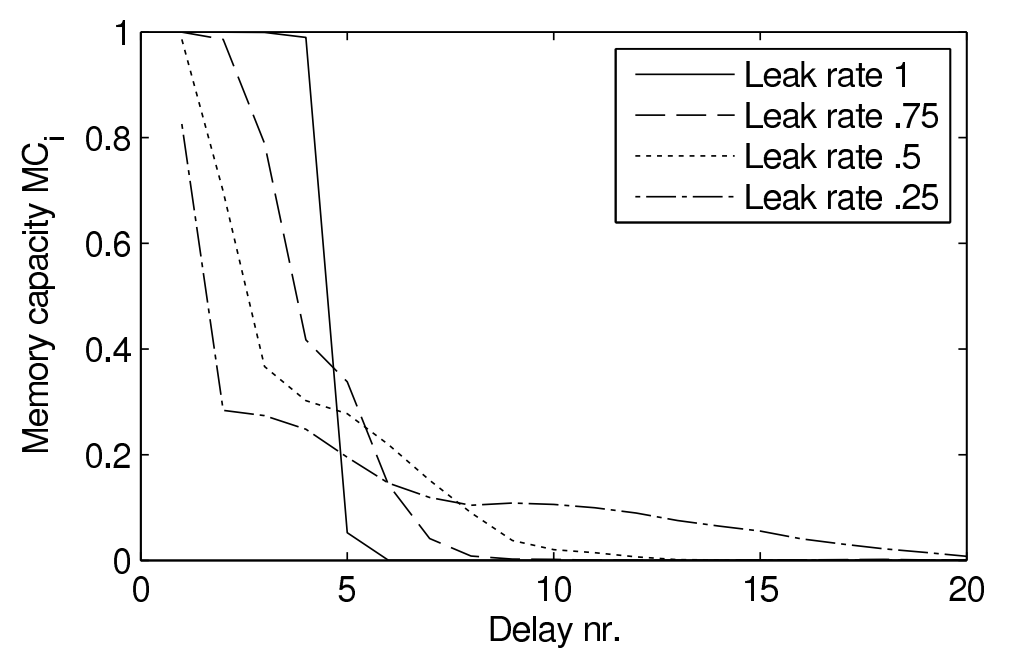
\includegraphics[width=0.55\textwidth]{img/leak_rate_verstraeten.png}
	
	\caption[Memory capacity for \acrshort{esn}s with different leak rates (from \citet{verstraeten_towards_2009}).]{
    		Memory capacity for \acrshort{esn}s with different leak rates (see Subsection \ref{subsection:esn}). Networks with a smaller leak rate show better long-term memory at the cost of decreased accuracy in short-term memory. This figure originally appeared in \citet{verstraeten_towards_2009}.
        }
	\label{fig:leak_rate_verstraeten}
\end{figure}


% This is shown in Figure 3.2. In this plot, the memory curve for a reservoir of 20 tanh nodes
% is shown with dierent leak rates. The plot shows that decreasing leak
% rates cause the memory curve to become flatter and wider. This means
% that the reservoir has worse memory of recent inputs, but better memory of inputs further in the past. Thus, by decreasing the leak rate we
% increase the longer-term memory of the nodes at the expense of precision
% in recalling the more recent inputs.


% Takeaway for reservoir computing
The takeaway here is that the time scale of the reservoir dynamics plays a vital role in its ability to solve a given task. 
A reservoir highly synchronized to its inputs will display faster dynamics and thus a shorter but greater precision integration window for solving tasks.
Conversely, a reservoir with higher memory capacity will typically exhibit slower dynamics and thus a longer integration window, at the expense of short-term precision.


\subsection{Sampling of a Continuous-Time Reservoir}

% What is the problem when sampling a continuous-time signal?
While the dynamics of a physical reservoir operate in continuous time, most applications implement the readout model digitally using a conventional computer and sensors that discretely sample the input signals and reservoir state.
According to the Shannon-Nyquist sampling theorem, to sample a continuous signal without losing information we must sample at twice the rate of the largest frequency component present in that signal \citep{shannon_communication_1949}.
Hence, determining the right time scale at which the desired reservoir dynamics occur plays a prominent role in PRC system design. 
Undersampling critical signals in the reservoir will result in information loss by introducing aliasing in the sampled signal. 
In conclusion, effectively sampling the reservoir state presents an additional optimization problem when implementing RC with physical reservoirs.


% What are the problems with undersampling or oversampling?
% Sampling at a higher frequency than the reservoir dynamics that can solve the desired task adds high-frequency noise to the signal. 
% The presence of this additive noise can degrade the performance of the linear readout function. 


% - TODO: Maybe here I can add a figure that is a toy demonstration of under and oversampling in an RC system?

